\documentclass[twoside]{book}

% Packages required by doxygen
\usepackage{fixltx2e}
\usepackage{calc}
\usepackage{doxygen}
\usepackage[export]{adjustbox} % also loads graphicx
\usepackage{graphicx}
\usepackage[utf8]{inputenc}
\usepackage{makeidx}
\usepackage{multicol}
\usepackage{multirow}
\PassOptionsToPackage{warn}{textcomp}
\usepackage{textcomp}
\usepackage[nointegrals]{wasysym}
\usepackage[table]{xcolor}

% Font selection
\usepackage[T1]{fontenc}
\usepackage[scaled=.90]{helvet}
\usepackage{courier}
\usepackage{amssymb}
\usepackage{sectsty}
\renewcommand{\familydefault}{\sfdefault}
\allsectionsfont{%
  \fontseries{bc}\selectfont%
  \color{darkgray}%
}
\renewcommand{\DoxyLabelFont}{%
  \fontseries{bc}\selectfont%
  \color{darkgray}%
}
\newcommand{\+}{\discretionary{\mbox{\scriptsize$\hookleftarrow$}}{}{}}

% Page & text layout
\usepackage{geometry}
\geometry{%
  a4paper,%
  top=2.5cm,%
  bottom=2.5cm,%
  left=2.5cm,%
  right=2.5cm%
}
\tolerance=750
\hfuzz=15pt
\hbadness=750
\setlength{\emergencystretch}{15pt}
\setlength{\parindent}{0cm}
\setlength{\parskip}{3ex plus 2ex minus 2ex}
\makeatletter
\renewcommand{\paragraph}{%
  \@startsection{paragraph}{4}{0ex}{-1.0ex}{1.0ex}{%
    \normalfont\normalsize\bfseries\SS@parafont%
  }%
}
\renewcommand{\subparagraph}{%
  \@startsection{subparagraph}{5}{0ex}{-1.0ex}{1.0ex}{%
    \normalfont\normalsize\bfseries\SS@subparafont%
  }%
}
\makeatother

% Headers & footers
\usepackage{fancyhdr}
\pagestyle{fancyplain}
\fancyhead[LE]{\fancyplain{}{\bfseries\thepage}}
\fancyhead[CE]{\fancyplain{}{}}
\fancyhead[RE]{\fancyplain{}{\bfseries\leftmark}}
\fancyhead[LO]{\fancyplain{}{\bfseries\rightmark}}
\fancyhead[CO]{\fancyplain{}{}}
\fancyhead[RO]{\fancyplain{}{\bfseries\thepage}}
\fancyfoot[LE]{\fancyplain{}{}}
\fancyfoot[CE]{\fancyplain{}{}}
\fancyfoot[RE]{\fancyplain{}{\bfseries\scriptsize Generated by Doxygen }}
\fancyfoot[LO]{\fancyplain{}{\bfseries\scriptsize Generated by Doxygen }}
\fancyfoot[CO]{\fancyplain{}{}}
\fancyfoot[RO]{\fancyplain{}{}}
\renewcommand{\footrulewidth}{0.4pt}
\renewcommand{\chaptermark}[1]{%
  \markboth{#1}{}%
}
\renewcommand{\sectionmark}[1]{%
  \markright{\thesection\ #1}%
}

% Indices & bibliography
\usepackage{natbib}
\usepackage[titles]{tocloft}
\setcounter{tocdepth}{3}
\setcounter{secnumdepth}{5}
\makeindex

% Hyperlinks (required, but should be loaded last)
\usepackage{ifpdf}
\ifpdf
  \usepackage[pdftex,pagebackref=true]{hyperref}
\else
  \usepackage[ps2pdf,pagebackref=true]{hyperref}
\fi
\hypersetup{%
  colorlinks=true,%
  linkcolor=blue,%
  citecolor=blue,%
  unicode%
}

% Custom commands
\newcommand{\clearemptydoublepage}{%
  \newpage{\pagestyle{empty}\cleardoublepage}%
}

\usepackage{caption}
\captionsetup{labelsep=space,justification=centering,font={bf},singlelinecheck=off,skip=4pt,position=top}

%===== C O N T E N T S =====

\begin{document}

% Titlepage & ToC
\hypersetup{pageanchor=false,
             bookmarksnumbered=true,
             pdfencoding=unicode
            }
\pagenumbering{alph}
\begin{titlepage}
\vspace*{7cm}
\begin{center}%
{\Large tttrlib \\[1ex]\large @ }\\
\vspace*{1cm}
{\large Generated by Doxygen 1.8.13}\\
\end{center}
\end{titlepage}
\clearemptydoublepage
\pagenumbering{roman}
\tableofcontents
\clearemptydoublepage
\pagenumbering{arabic}
\hypersetup{pageanchor=true}

%--- Begin generated contents ---
\chapter{C\+H\+A\+N\+G\+ES}
\label{md__c_h_a_n_g_e_s}
\Hypertarget{md__c_h_a_n_g_e_s}
\input{md__c_h_a_n_g_e_s}
\chapter{tttrlib}
\label{md__r_e_a_d_m_e}
\Hypertarget{md__r_e_a_d_m_e}
\href{https://travis-ci.org/tpeulen/tttrlib}{\tt } \href{https://anaconda.org/tpeulen/tttrlib}{\tt } \href{https://anaconda.org/tpeulen/tttrlib}{\tt } \href{https://www.codacy.com?utm_source=github.com&amp;utm_medium=referral&amp;utm_content=tpeulen/tttrlib&amp;utm_campaign=Badge_Grade}{\tt }

\subsection*{General description}

tttrlib is a file format agnostic low level, high performance A\+PI to read and process time-\/tagged-\/time resolved (T\+T\+TR) data acquired by Pico\+Quant (PQ) and Becker\&Hickl measurement devices/cards or T\+T\+TR files in the open Photon-\/\+H\+DF format.

The library tttrlib facilitates the work with files containing time-\/tagged time resolved photon streams by providing a vendor independent C++ application programming interface (A\+PI) for T\+T\+TR files that is wrapped by S\+W\+IG (Simplified Wrapper and Interface Generator) for common scripting languages as Python as target languages and non-\/scripting languages such as C\# and Java including Octave, Scilab and R.


\begin{DoxyItemize}
\item Multi-\/dimensional histograms
\item Correlation analysis
\item Time-\/window analysis
\item Photon distribution anaylsis
\item F\+L\+IM image generation and analysis
\end{DoxyItemize}



tttrlib is N\+OT intended as ready-\/to-\/use software for specific application purposes.

\subsection*{Supported file formats}

\subsubsection*{Pico\+Quant (PQ)}


\begin{DoxyItemize}
\item Pico\+Harp ptu, T2/\+T3
\item Hydra\+Harp ptu, T2/\+T3
\item Hydra\+Harp ht3, P\+TU
\end{DoxyItemize}

\subsubsection*{Becker \& Hickl (BH)}


\begin{DoxyItemize}
\item spc132
\item spc630 (256 \& 4096 mode)
\end{DoxyItemize}

\subsection*{Design goals}


\begin{DoxyItemize}
\item Low memory footprint (keep objective large datasets, e.\+g. F\+L\+IM in memory). Particulary useful for F\+L\+IM.
\item Platform independent C/\+C++ library with interfaces for scripting libraries
\end{DoxyItemize}

\subsection*{Capabilities}


\begin{DoxyItemize}
\item Fast (IO limited) Reading T\+T\+TR files
\item Generation / analysis of fluorescence decays
\item Time window analysis
\item Correlation of time event traces
\item Filtering of time event traces to generate instrument response functions for fluorescence decays analysis without the need of independent measurements..
\item Fast photon distribution analysis
\item Fast selection of photons from a photon stream
\end{DoxyItemize}

Generation of fluorescence decay histograms tttrlib outperforms pure numpy and Python based libraries by a factor of $\sim$40

\subsection*{Implementation}

Pure pure C/\+C++ and C\+U\+DA based high performance algorithms for real-\/time and interactive analysis of T\+T\+TR data.

\section*{Building and Installation}

\subsection*{C++ shared library}

The C++ shared library can be installed from source with \href{https://cmake.org/}{\tt cmake}\+:


\begin{DoxyCode}
git clone --recursive https://github.com/tpeulen/tttrlib.git
mkdir tttrlib/build; cd tttrlib/build
cmake ..
sudo make install
\end{DoxyCode}


On Linux you can build and install a package instead (prefered)\+:

\subsection*{Python bindings}

The Python bindings can be either be installed by downloading and compiling the source code or by using a precompiled distribution for Python anaconda environment.

The following commands can be used to download and compile the source code\+:


\begin{DoxyCode}
git clone --recursive https://github.com/tpeulen/tttrlib.git
cd tttrlib
sudo python setup.py install
\end{DoxyCode}


In an \href{https://www.anaconda.com/}{\tt anaconda} environment the library can be installed by the following command\+: 
\begin{DoxyCode}
conda install -c tpeulen tttrlib
\end{DoxyCode}


For most users the later approach is recommended. Currently, pre-\/compiled packages for the anaconda distribution system are available for\+:


\begin{DoxyItemize}
\item Windows\+: Python 2.\+7, Python 3.\+7 (x64)
\item Linux\+: Python 2.\+7, Python 3.\+7 (x64)
\item Mac\+Os\+: Python 2.\+7 (x64)
\end{DoxyItemize}

Legacy 32-\/bit platforms are currently not supported.

\section*{Documentation}

The A\+PI of tttrlib as well as some use cases are documented on its \href{https://tpeulen.github.io/tttrlib}{\tt web page}

Note, tttrlib is highly experimental library in current development. In case you notice unusual behaviour do not hesitate to contact the authors.

\section*{License}

tttrlib is released under the open source M\+IT license. 
\chapter{Roadmap}
\label{md__t_o_d_o}
\Hypertarget{md__t_o_d_o}
\input{md__t_o_d_o}
\chapter{Namespace Index}
\input{namespaces}
\chapter{Hierarchical Index}
\section{Class Hierarchy}
This inheritance list is sorted roughly, but not completely, alphabetically\+:\begin{DoxyCompactList}
\item \contentsline{section}{Axis$<$ T $>$}{\pageref{class_axis}}{}
\item \contentsline{section}{bh\+\_\+overflow\+\_\+t}{\pageref{unionbh__overflow__t}}{}
\item \contentsline{section}{bh\+\_\+spc130\+\_\+overflow\+\_\+t}{\pageref{unionbh__spc130__overflow__t}}{}
\item \contentsline{section}{bh\+\_\+spc130\+\_\+record\+\_\+t}{\pageref{unionbh__spc130__record__t}}{}
\item \contentsline{section}{bh\+\_\+spc600\+\_\+256\+\_\+overflow\+\_\+t}{\pageref{unionbh__spc600__256__overflow__t}}{}
\item \contentsline{section}{bh\+\_\+spc600\+\_\+256\+\_\+record\+\_\+t}{\pageref{unionbh__spc600__256__record__t}}{}
\item \contentsline{section}{bh\+\_\+spc600\+\_\+4096\+\_\+record\+\_\+t}{\pageref{unionbh__spc600__4096__record__t}}{}
\item \contentsline{section}{Curve\+Mapping\+\_\+t}{\pageref{struct_curve_mapping__t}}{}
\item \contentsline{section}{Header}{\pageref{class_header}}{}
\item \contentsline{section}{Histogram$<$ T $>$}{\pageref{class_histogram}}{}
\item \contentsline{section}{Param\+Struct\+\_\+t}{\pageref{struct_param_struct__t}}{}
\item \contentsline{section}{pq\+\_\+hh\+\_\+t2\+\_\+record\+\_\+t}{\pageref{unionpq__hh__t2__record__t}}{}
\item \contentsline{section}{pq\+\_\+hh\+\_\+t3\+\_\+record\+\_\+t}{\pageref{unionpq__hh__t3__record__t}}{}
\item \contentsline{section}{pq\+\_\+ht3\+\_\+ascii\+\_\+t}{\pageref{structpq__ht3__ascii__t}}{}
\item \contentsline{section}{pq\+\_\+ht3\+\_\+\+Bin\+Hdr\+\_\+t}{\pageref{structpq__ht3___bin_hdr__t}}{}
\item \contentsline{section}{pq\+\_\+ht3\+\_\+board\+\_\+settings\+\_\+t}{\pageref{structpq__ht3__board__settings__t}}{}
\item \contentsline{section}{pq\+\_\+ht3\+\_\+\+Board\+Hdr}{\pageref{structpq__ht3___board_hdr}}{}
\item \contentsline{section}{pq\+\_\+ht3\+\_\+\+T\+T\+T\+R\+Hdr}{\pageref{structpq__ht3___t_t_t_r_hdr}}{}
\item \contentsline{section}{pq\+\_\+ph\+\_\+t2\+\_\+record\+\_\+t}{\pageref{unionpq__ph__t2__record__t}}{}
\item \contentsline{section}{pq\+\_\+ph\+\_\+t3\+\_\+record\+\_\+t}{\pageref{unionpq__ph__t3__record__t}}{}
\item \contentsline{section}{tag\+\_\+head\+\_\+t}{\pageref{structtag__head__t}}{}
\item \contentsline{section}{T\+T\+TR}{\pageref{class_t_t_t_r}}{}
\begin{DoxyCompactList}
\item \contentsline{section}{S\+PC}{\pageref{class_s_p_c}}{}
\end{DoxyCompactList}
\item \contentsline{section}{T\+T\+T\+R\+Reader}{\pageref{class_t_t_t_r_reader}}{}
\end{DoxyCompactList}

\chapter{Class Index}
\section{Class List}
Here are the classes, structs, unions and interfaces with brief descriptions\+:\begin{DoxyCompactList}
\item\contentsline{section}{\hyperlink{class_axis}{Axis$<$ T $>$} }{\pageref{class_axis}}{}
\item\contentsline{section}{\hyperlink{unionbh__overflow__t}{bh\+\_\+overflow\+\_\+t} \\*Becker Hickl S\+P\+C-\/130/600 macro time overflow record }{\pageref{unionbh__overflow__t}}{}
\item\contentsline{section}{\hyperlink{unionbh__spc130__record__t}{bh\+\_\+spc130\+\_\+record\+\_\+t} \\*Becker Hickl S\+P\+C-\/130, regular record }{\pageref{unionbh__spc130__record__t}}{}
\item\contentsline{section}{\hyperlink{unionbh__spc600__256__record__t}{bh\+\_\+spc600\+\_\+256\+\_\+record\+\_\+t} \\*Becker Hickl S\+P\+C-\/600/630 256 Channel Mode, regular record }{\pageref{unionbh__spc600__256__record__t}}{}
\item\contentsline{section}{\hyperlink{unionbh__spc600__4096__record__t}{bh\+\_\+spc600\+\_\+4096\+\_\+record\+\_\+t} \\*Becker Hickl S\+P\+C-\/600/630 4096 Channel Mode }{\pageref{unionbh__spc600__4096__record__t}}{}
\item\contentsline{section}{\hyperlink{class_correlator}{Correlator} }{\pageref{class_correlator}}{}
\item\contentsline{section}{\hyperlink{struct_curve_mapping__t}{Curve\+Mapping\+\_\+t} }{\pageref{struct_curve_mapping__t}}{}
\item\contentsline{section}{\hyperlink{class_header}{Header} }{\pageref{class_header}}{}
\item\contentsline{section}{\hyperlink{class_histogram}{Histogram$<$ T $>$} }{\pageref{class_histogram}}{}
\item\contentsline{section}{\hyperlink{struct_param_struct__t}{Param\+Struct\+\_\+t} }{\pageref{struct_param_struct__t}}{}
\item\contentsline{section}{\hyperlink{unionpq__hh__t2__record__t}{pq\+\_\+hh\+\_\+t2\+\_\+record\+\_\+t} \\*Hydra\+Harp/\+Time\+Harp260 T2 record }{\pageref{unionpq__hh__t2__record__t}}{}
\item\contentsline{section}{\hyperlink{unionpq__hh__t3__record__t}{pq\+\_\+hh\+\_\+t3\+\_\+record\+\_\+t} \\*Hydra\+Harp/\+Time\+Harp260 T3 record }{\pageref{unionpq__hh__t3__record__t}}{}
\item\contentsline{section}{\hyperlink{structpq__ht3__ascii__t}{pq\+\_\+ht3\+\_\+ascii\+\_\+t} \\*The following represents the readable A\+S\+C\+II file header portion }{\pageref{structpq__ht3__ascii__t}}{}
\item\contentsline{section}{\hyperlink{structpq__ht3___bin_hdr__t}{pq\+\_\+ht3\+\_\+\+Bin\+Hdr\+\_\+t} \\*The following is binary file header information }{\pageref{structpq__ht3___bin_hdr__t}}{}
\item\contentsline{section}{\hyperlink{structpq__ht3__board__settings__t}{pq\+\_\+ht3\+\_\+board\+\_\+settings\+\_\+t} }{\pageref{structpq__ht3__board__settings__t}}{}
\item\contentsline{section}{\hyperlink{structpq__ht3___board_hdr}{pq\+\_\+ht3\+\_\+\+Board\+Hdr} }{\pageref{structpq__ht3___board_hdr}}{}
\item\contentsline{section}{\hyperlink{structpq__ht3___t_t_t_r_hdr}{pq\+\_\+ht3\+\_\+\+T\+T\+T\+R\+Hdr} }{\pageref{structpq__ht3___t_t_t_r_hdr}}{}
\item\contentsline{section}{\hyperlink{unionpq__ph__t2__record__t}{pq\+\_\+ph\+\_\+t2\+\_\+record\+\_\+t} \\*Pico\+Harp T2 input }{\pageref{unionpq__ph__t2__record__t}}{}
\item\contentsline{section}{\hyperlink{unionpq__ph__t3__record__t}{pq\+\_\+ph\+\_\+t3\+\_\+record\+\_\+t} \\*Pico\+Harp T3 input }{\pageref{unionpq__ph__t3__record__t}}{}
\item\contentsline{section}{\hyperlink{structtag__head__t}{tag\+\_\+head\+\_\+t} \\*A \hyperlink{class_header}{Header} Tag entry of a P\+TU file }{\pageref{structtag__head__t}}{}
\item\contentsline{section}{\hyperlink{class_t_t_t_r}{T\+T\+TR} }{\pageref{class_t_t_t_r}}{}
\item\contentsline{section}{\hyperlink{class_t_t_t_r_reader}{T\+T\+T\+R\+Reader} }{\pageref{class_t_t_t_r_reader}}{}
\end{DoxyCompactList}

\chapter{File Index}
\section{File List}
Here is a list of all files with brief descriptions\+:\begin{DoxyCompactList}
\item\contentsline{section}{\hyperlink{correlate_8h}{correlate.\+h} \\*File containing example of doxygen usage for quick reference }{\pageref{correlate_8h}}{}
\item\contentsline{section}{\hyperlink{_header_8h}{Header.\+h} }{\pageref{_header_8h}}{}
\item\contentsline{section}{\hyperlink{_histogram_8h}{Histogram.\+h} }{\pageref{_histogram_8h}}{}
\item\contentsline{section}{\hyperlink{_record_reader_8h}{Record\+Reader.\+h} }{\pageref{_record_reader_8h}}{}
\item\contentsline{section}{\hyperlink{_t_t_t_r_8h}{T\+T\+T\+R.\+h} }{\pageref{_t_t_t_r_8h}}{}
\item\contentsline{section}{\hyperlink{_t_t_t_r_reader_8h}{T\+T\+T\+R\+Reader.\+h} }{\pageref{_t_t_t_r_reader_8h}}{}
\end{DoxyCompactList}

\chapter{Namespace Documentation}
\input{namespacescratch}
\input{namespacesetup}
\chapter{Class Documentation}
\hypertarget{classsetup_1_1_c_make_build}{}\doxysection{setup.\+C\+Make\+Build Class Reference}
\label{classsetup_1_1_c_make_build}\index{setup.CMakeBuild@{setup.CMakeBuild}}
Inheritance diagram for setup.\+C\+Make\+Build\+:\begin{figure}[H]
\begin{center}
\leavevmode
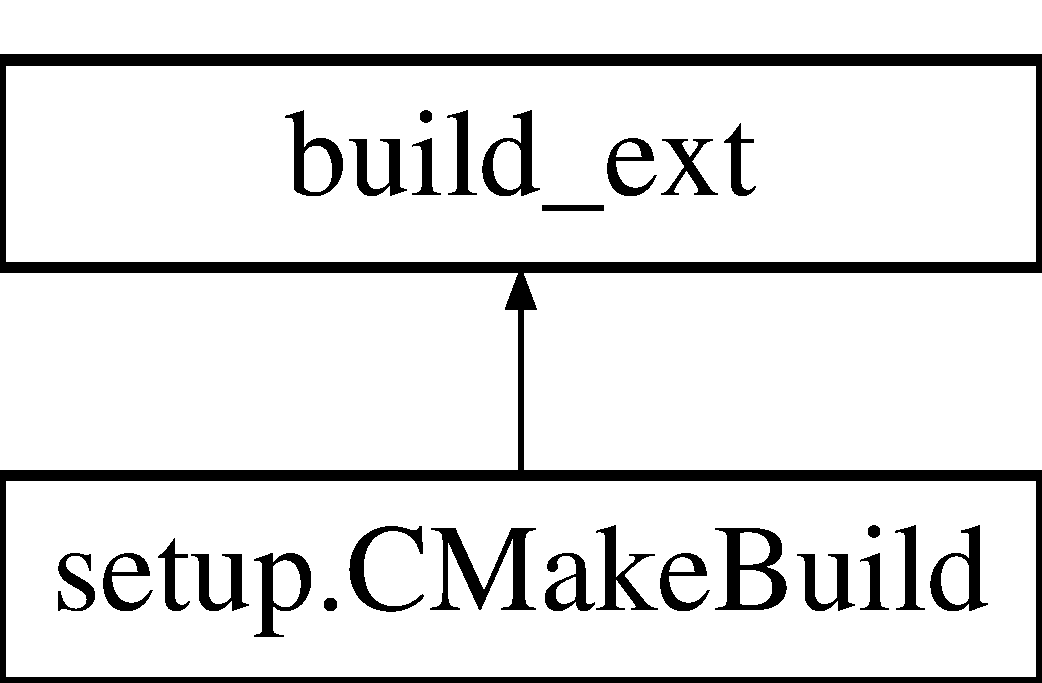
\includegraphics[height=2.000000cm]{classsetup_1_1_c_make_build}
\end{center}
\end{figure}
\doxysubsection*{Public Member Functions}
\begin{DoxyCompactItemize}
\item 
\mbox{\Hypertarget{classsetup_1_1_c_make_build_aaeaa47a0e82fe56564dd8cec58f772c9}\label{classsetup_1_1_c_make_build_aaeaa47a0e82fe56564dd8cec58f772c9}} 
def {\bfseries run} (self)
\item 
\mbox{\Hypertarget{classsetup_1_1_c_make_build_a7b078d0cd6b68f830254e3d96a9e96b1}\label{classsetup_1_1_c_make_build_a7b078d0cd6b68f830254e3d96a9e96b1}} 
def {\bfseries build\+\_\+extension} (self, ext)
\end{DoxyCompactItemize}


The documentation for this class was generated from the following file\+:\begin{DoxyCompactItemize}
\item 
setup.\+py\end{DoxyCompactItemize}

\hypertarget{classsetup_1_1_c_make_extension}{}\doxysection{setup.\+C\+Make\+Extension Class Reference}
\label{classsetup_1_1_c_make_extension}\index{setup.CMakeExtension@{setup.CMakeExtension}}
Inheritance diagram for setup.\+C\+Make\+Extension\+:\begin{figure}[H]
\begin{center}
\leavevmode
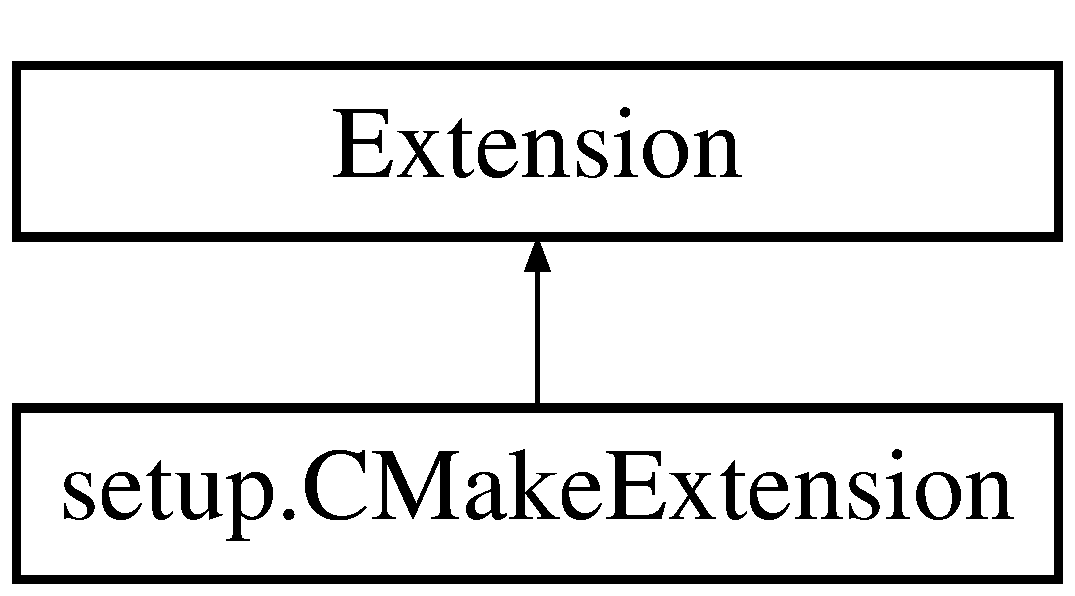
\includegraphics[height=2.000000cm]{classsetup_1_1_c_make_extension}
\end{center}
\end{figure}
\doxysubsection*{Public Member Functions}
\begin{DoxyCompactItemize}
\item 
\mbox{\Hypertarget{classsetup_1_1_c_make_extension_a2e49eec9170175d7c21d338bad44c6aa}\label{classsetup_1_1_c_make_extension_a2e49eec9170175d7c21d338bad44c6aa}} 
def {\bfseries \+\_\+\+\_\+init\+\_\+\+\_\+} (self, name, sourcedir=\textquotesingle{}\textquotesingle{})
\end{DoxyCompactItemize}
\doxysubsection*{Public Attributes}
\begin{DoxyCompactItemize}
\item 
\mbox{\Hypertarget{classsetup_1_1_c_make_extension_a29a643870fbe57b4181a02fb4d57b9f7}\label{classsetup_1_1_c_make_extension_a29a643870fbe57b4181a02fb4d57b9f7}} 
{\bfseries sourcedir}
\end{DoxyCompactItemize}


The documentation for this class was generated from the following file\+:\begin{DoxyCompactItemize}
\item 
setup.\+py\end{DoxyCompactItemize}

\chapter{File Documentation}
\input{_c_h_a_n_g_e_s_8md}
\input{_r_e_a_d_m_e_8md}
\input{scratch_8py}
\input{setup_8py}
\input{_t_o_d_o_8md}
%--- End generated contents ---

% Index
\backmatter
\newpage
\phantomsection
\clearemptydoublepage
\addcontentsline{toc}{chapter}{Index}
\printindex

\end{document}
